	%%%%%START-of-DOCUMENT%%%%%%%%%%%%%%%
\documentclass[11pt]{article}
\usepackage{amsmath,amssymb,amsthm}
\usepackage{hyperref}
\usepackage{graphicx}
\usepackage[margin=1in]{geometry}
\usepackage{fancyhdr}
\usepackage{mathtools}
\usepackage{qtree}
\DeclarePairedDelimiter\ceil{\lceil}{\rceil}
\DeclarePairedDelimiter\floor{\lfloor}{\rfloor}
\setlength{\parindent}{0pt}
\setlength{\parskip}{5pt plus 1pt}
\setlength{\headheight}{13.6pt}
\newcommand{\sep}{\hspace*{.5em}}
\newcommand\question[3]{\vspace{.25in}\textbf{#1: #2}\vspace{.5em}\hrule\vspace{.10in}}
\renewcommand\part[1]{\vspace{.10in}\textbf{(#1)}}
\newcommand\algorithm{\vspace{.10in}\textbf{Complexity: }}
\newcommand\correctness{\vspace{.10in}\textbf{Correctness: }}
\newcommand\runtime{\vspace{.10in}\textbf{Running time: }}
\pagestyle{fancyplain}
\lhead{{\NAME\ (\BID) (\SECTION)}}
%\chead{\textbf{HW\HWNUM}}
\rhead{\today}

\begin{document}\raggedright
\title{CS 575\\Homework 2}
\date{}
\maketitle
“I have done this assignment completely on my own. I have not
copied it, nor have I given my solution to anyone else. I under-
stand that if I am involved in plagiarism or cheating I will have
to sign an official form that I have cheated and that this form will
be stored in my official university record. I also understand that
I will receive a grade of 0 for the involved assignment for my first
offense and that I will receive a grade of “F” for the course for any
additional offense.”
\begin{flushright}
	\hspace{12cm} Sign : \hrulefill
\end{flushright}
%Section A==============Change the values below to match your information==================
\newcommand\NAME{Aniruddha Tekade}  	% your name
\newcommand\BID{B00618834}     	% your andrew id
\newcommand\SECTION{Section-02}   % your section-02.
\newcommand\HWNUM{2}              	% the homework number
%Section B==============Put your answers to the questions below here=======================
% no need to restate the problem --- the graders know which problem is which, but replacing "The First Problem" with a short phrase will help you remember which problem this is when you read over your homeworks to study.
%==========================================================================================
%==========================================================================================

\question{1}{You are given an input array of integers: [8, 3, 7, 1, 2, 10, 5]} 

\part{a} The \texttt{max-heap} build process stepwise : 
\begin{itemize}
	\item Step I $\Rightarrow$
 		\Tree[.8 
				[.3 
					[.1 ][.2 ] 
				] 
				[.7 
					[.10 ][.5 ] 
				]
			]
	\item Step II $\Rightarrow$
		\Tree[.8 
				[.3 
					[.1 ][.2 ] 
				] 
				[.10 
					[.7 ][.5 ] 
				]
			]
	\item Step III $\Rightarrow$
		\Tree[.10 
				[.3 
					[.1 ][.2 ] 
				] 
				[.8 
					[.7 ][.5 ] 
				]
			]
\end{itemize}

\part{b} The non-descending heapsort algorithm steps :

\begin{itemize}
	\item Step I $\Rightarrow$ \\
	\texttt{Map-Heap} array represention : 
	\noindent
  $\fbox{5} \sep \fbox{3} \sep \fbox{8} \sep \fbox{1} \sep \fbox{2} \sep \fbox{7} \sep \fbox{10}$ 
  \newline \\
  Heap after swapping 5 \& 10 : 
   \Tree[.5 
				[.3 
					[.1 ][.2 ] 
				] 
				[.8 
					[.7 ][.10 ] 
				]
			]
  \newline \\ Remove last element from heap, insert it into the destination array \& reduce size of heap by 1. \texttt{Map-Heap} array represention : 
	\noindent
  $\fbox{5} \sep \fbox{3} \sep \fbox{8} \sep \fbox{1} \sep \fbox{2} \sep \fbox{7}$
  \newline
  Destination Array : 
  \noindent
  $\fbox{10}$ 
  \\ 
  Max-Heap after heapify: 
   \Tree[.8 
				[.3 
					[.1 ][.2 ] 
				] 
				[.7 
					[.5 ] 
				]
			]
	
	\item Step II $\Rightarrow$ \\
	\texttt{Map-Heap} array represention : 
	\noindent
  $\fbox{8} \sep \fbox{3} \sep \fbox{1} \sep \fbox{2} \sep \fbox{7} \sep \fbox{5}$ 
  \newline \\
  Heap after swapping 5 \& 8 : 
   \Tree[.5 
				[.3 
					[.1 ][.2 ] 
				] 
				[.7 
					[.8 ] 
				]
			]
  \newline \\ Remove last element from heap, insert it into the destination array \& reduce size of heap by 1. \texttt{Map-Heap} array represention : 
	\noindent
  $\fbox{5} \sep \fbox{3} \sep \fbox{1} \sep \fbox{2} \sep \fbox{7}$
  \newline
  Destination Array : 
  \noindent
  $\fbox{10} \sep \fbox{8}$ 
  \\ 
  Max-Heap after heapify: 
   \Tree[.7 
				[.3 
					[.1 ][.2 ] 
				] 
				[.5 ]
			]
	
	\item Step III $\Rightarrow$ \\
	\texttt{Map-Heap} array represention : 
	\noindent
  $\fbox{7} \sep \fbox{3} \sep \fbox{5} \sep \fbox{1} \sep \fbox{2}$ 
  \newline \\
  Heap after swapping 2 \& 7 : 
   \Tree[.2 
				[.3 
					[.1 ][.7 ] 
				] 
				[.5 ]
			]
  \newline \\ Remove last element from heap, insert it into the destination array \& reduce size of heap by 1. \texttt{Map-Heap} array represention : 
	\noindent
  $\fbox{2} \sep \fbox{3} \sep \fbox{5} \sep \fbox{1}$
  \newline
  Destination Array : 
  \noindent
  $\fbox{10} \sep \fbox{8} \sep \fbox{7}$ 
  \\ 
  Max-Heap after heapify: 
   \Tree[.5 
				[.2 
					[.1 ] 
				] 
				[.3 ]
			]
	
	\item Step IV $\Rightarrow$ \\
	\texttt{Map-Heap} array represention : 
	\noindent
  $\fbox{5} \sep \fbox{2} \sep \fbox{3} \sep \fbox{1}$ 
  \newline \\
  Heap after swapping 1 \& 5 : 
   \Tree[.1 
				[.2 
					[.5 ] 
				] 
				[.3 ]
			]
  \newline \\ Remove last element from heap, insert it into the destination array \& reduce size of heap by 1. \texttt{Map-Heap} array represention : 
	\noindent
  $\fbox{1} \sep \fbox{2} \sep \fbox{3}$
  \newline
  Destination Array : 
  \noindent
  $\fbox{10} \sep \fbox{8} \sep \fbox{7} \sep \fbox{5}$ 
  \\ 
  Max-Heap after heapify: 
   \Tree[.3 [.1 ][.2 ] ]
			
	\item Step V $\Rightarrow$ \\
		\texttt{Map-Heap} array represention : 
		\noindent
  			$\fbox{3} \sep \fbox{1} \sep \fbox{2}$ 
  		\newline \\
  		Heap after swapping 2 \& 3 : 
   		\Tree[.1 [.2 ][.3 ] ]
 		\newline \\ Remove last element from heap, insert it into the destination array \& 		reduce size of heap by 1. \texttt{Map-Heap} array represention : 
		\noindent
  		$\fbox{2} \sep \fbox{1}$
  		\newline
  		Destination Array : 
  		\noindent
	  	$\fbox{10} \sep \fbox{8} \sep \fbox{7} \sep \fbox{5} \sep \fbox{3}$ 
  		\\ 
  		Max-Heap after heapify: 
   		\Tree[.2 [.1 ] ]
   	\item Step VI $\Rightarrow$ \\
		\texttt{Map-Heap} array represention : 
		\noindent
  			$\fbox{2} \sep \fbox{1}$ 
  		\newline \\
  		Heap after swapping 1 \& 2 : 
   		\Tree[.1 [.2 ] ]
 		\newline \\ Remove last element from heap, insert it into the destination array \& 		reduce size of heap by 1. \texttt{Map-Heap} array represention : 
		\noindent
  		$\fbox{1}$
  		\newline
  		Destination Array : 
  		\noindent
	  	$\fbox{10} \sep \fbox{8} \sep \fbox{7} \sep \fbox{5} \sep \fbox{3} \sep \fbox{2}$ 
  		\\ 
  	Max-Heap after heapify: 
   		\Tree[.1 ]
   	\item Insert the element into the destination array. The final non-descending array will look like this $\Rightarrow$ 
   	\noindent
	  	$\fbox{10} \sep \fbox{8} \sep \fbox{7} \sep \fbox{5} \sep \fbox{3} \sep \fbox{2} \sep \fbox{1}$
   	
\end{itemize}



  

%================================================================================

\question{2}{Assume that you are given an array of n elements sorted in non-descending order where n $\geq$ 1. Given the assumption, solve the following problem via divide and conquer.}

\part{a} Ternary search algorithms psuedocode $\Rightarrow$
\begin{verbatim}
1.  TernarySearch(low, high, S, x)
2.    if low > high then
3.        return NoSuchKey
4.    else 
5.        mid1 <-- low + (floor(high - low) / 3)
6.        if (x == S[mid1])
7.            return mid1
8.        mid2 <-- high - (floor(high - low) / 3)
9.        if (x == S[mid2])
10.           return mid2
11.       if (x < S[mid1])
12.           return TernarySearch(low, mid1 - 1, S, x)
13.       else if (x > S[mid2])
14.           return TernarySearch(mid2 + 1, high, S, x)
15.       else 
16.           return TernarySearch(mid1 + 1, mid2 - 1, S, x)
\end{verbatim}

\part{b} \textbf{Time complexity of Ternary Search algoriths is define by following recurrence definition} $\Rightarrow$
\[ T(n) = \begin{cases}
				0 & \text{if $n = 0$} \\
				1 & \text{if  $n = 1$} \\
				1 + T(n/3) & \text{if $n > 1$}
			\end{cases}
\]
Assume, input data size is n = $3^k$ \\
$\therefore$ k = $\log_3$ n\\
Solving the above equation \\
\hspace{5cm} $\Rightarrow$ T(n) = 1 + T(n/3) \\
\hspace{5cm} $\Rightarrow$ T(n/3) = 1 + 1 + T(n/9) = 2 + T(n/9)\\
\hspace{5cm} $\Rightarrow$ T(n/9) = 1 + 1 + 1 + T(n/27) = 3 + T(n/27)\\
\hspace{5cm} $\Rightarrow$ . . . \\
\hspace{5cm} $\Rightarrow$ . . . \\
\hspace{5cm} $\Rightarrow$ T(n/3) = k + T(n/$3^k$) = $\log_3 n$ + 1\\
 
Therefore, worst case time complexity of \texttt{TernarySearch} algorithms = $\Theta$($\log_3$n)
%=========================================================================================
\newpage
\question{3} {Use the radix sort algorithm to sort the following list of numbers in non-descending order: 321, 38, 15, 3, 9, 82, 10, 11.}

\part{a} \textbf{Explanation} $\Rightarrow$ The radix sort algorithsm working steps on the given input set are as follows:
\begin{itemize}
	\item Perform radix sort at unit's place of each element of input. \newline 
		\begin{figure}[h]
			\centering
			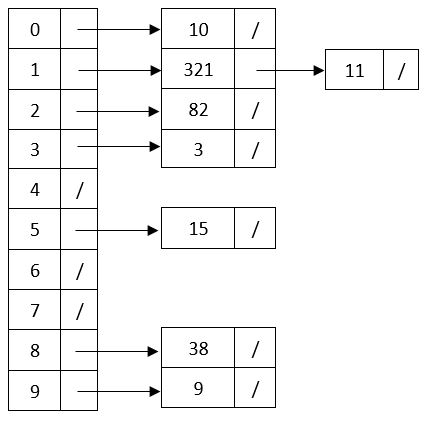
\includegraphics[width=65mm]{radixsort01.JPG}
			\caption{RadixSort Step(1) \label{overflow}}
		\end{figure}
		\\
		\textbf{Pass 1 $\Rightarrow$ 10, 321, 11, 82, 3, 15, 38, 9}
	\item Perform radix sort at ten's place of each element of pass 1
		\begin{figure}[h]
			\centering
			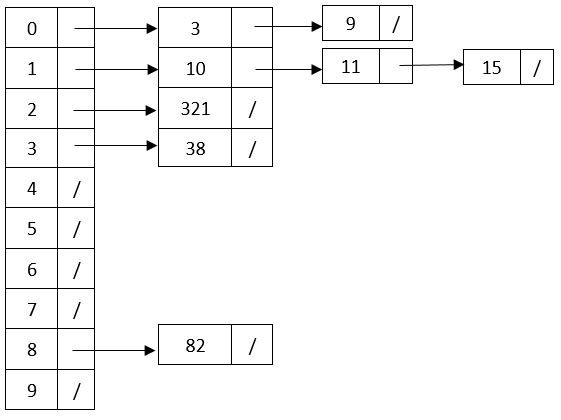
\includegraphics[width=70mm]{radixsort02.JPG}
			\caption{RadixSort Step(2) \label{overflow}}
		\end{figure}	
		\\
		\textbf{Pass 2 $\Rightarrow$ 3, 9, 10, 11, 15, 321, 38, 82}
	\item Perform radix sort at hundred's place of each element of pass 1
		\begin{figure}[h]
			\centering
			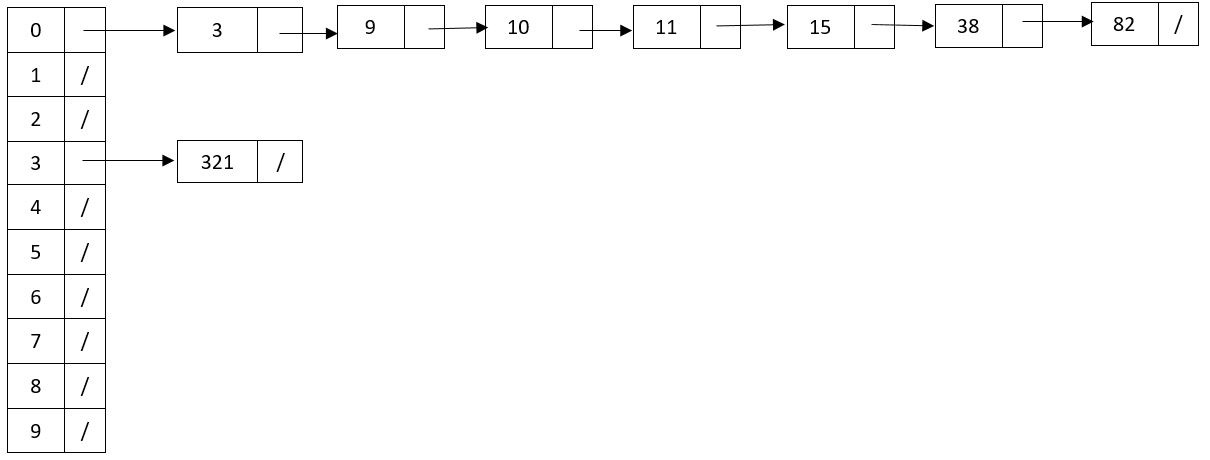
\includegraphics[width=140mm, height=60mm]{radixsort03.JPG}
			\caption{RadixSort Step(3) \label{overflow}}
		\end{figure}	
		\\
		\textbf{Pass 3 $\Rightarrow$ 3, 9, 10, 11, 15, 38, 82, 321}
\end{itemize} 
\newpage
\part{b} \textbf{Radix Sort using most signifincant digit first $\Rightarrow$} 

Unlike Radix sort with \texttt{least significant digit first}, Radix sort with \texttt{most significant digit first}, peforms the sorting in lexicographical order which is best suitable for set of characters, strings, words, very long integers \& alpabetical input data set. 
\newline \\
However, applying this technique on small integers may not work efficiently as after a centrain number of processing, it repeats the sorting output. This phenomenon can be realized using following diagrams $\Rightarrow$

\begin{itemize}
	\item Perform RadixSort MSD first : Step(I)
		\begin{figure}[h]
			\centering
			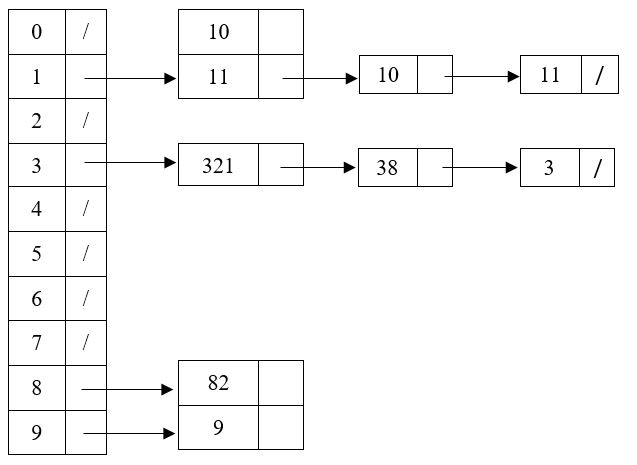
\includegraphics[width=70mm]{radixsortMSD01.JPG}
			\caption{RadixSort MSD first : Step(1) \label{overflow}}
		\end{figure}
		\\
		\textbf{Output after pass 1 $\Rightarrow$ 10, 15, 11, 321, 38, 3, 82, 9}
		\newpage
	\item Perform RadixSort MSD at each element of pass 1 : Step(II) \newline
		\begin{figure}[h]
			\centering
			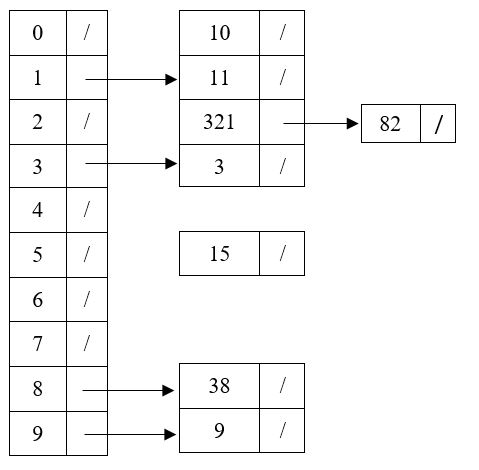
\includegraphics[width=70mm, height=65mm]{radixsortMSD02.JPG}
			\caption{RadixSort MSD first : Step(2) \label{overflow}}
		\end{figure}	
		\\
		\textbf{Pass 2 $\Rightarrow$ 10, 11, 321, 82, 3, 15, 38, 9}
	\item Perform radix sort at nest MSD of each element of pass 2
		\begin{figure}[h]
			\centering
			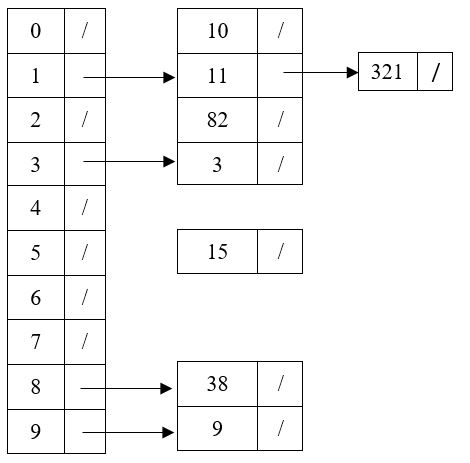
\includegraphics[width=70mm, height=60mm]{radixsortMSD03.JPG}
			\caption{RadixSort with MSD first : Step(3) \label{overflow}}
		\end{figure}	
		\\
		\textbf{Pass 3 $\Rightarrow$ 10, 11, 321, 82, 3, 15, 38, 9}
\end{itemize} 
And now, we can see that after pass 3 for every new interation, the same output will be returned since, for every new pass, same digit will be considered for sorting. 
\newline \\
Therefore, radix sort using most significant digit may not maintain the sorted order of input and may be inefficient for small size input. In short, it does not sort the small integers like given data set properly. 
\newline \\
Radix sort with \texttt{most significant digit first} should only be applied to integers where every element of the integer dataset have equal length.
%====================================================================================

\question{4} {Prove that the lower bound of sorting based on comparions is $\Omega$($nlgn$)}

\textbf{Explanation} $\Rightarrow$ 
\begin{itemize}
	\item When a list of n integers is given as input to sorting algorithm like heapsort (which is a comparison based sorting), the input data can be arranged in n! ways.
	\item We build a decision tree that has n! leaf nodes where each leaf could be a sorted permutation \& in each node of a decision tree, we compare two specific numbers at every interation or recursive call.
	\item Based on the result of the comparisons, we traverse to the left or right branch of the current node. 
	\item Depth of the decision tree indicates total number of comparisons to reach a sorted permutation. So mathematically $\Rightarrow$
	\begin{itemize}
		\item Depth = lg n! ; where n! is approximately $(n/e)^n$
		\item $\therefore$ lg n! = n lg$(n/e)$ which is $\Omega$(n lg n)
	\end{itemize}
	\item Therefore, the time complexity of sorting algorithms based on comparison is $\Omega$(n lg n).
\end{itemize}

 
 In each node of a decision tree, compare two specific numbers
 Based on the result of the comparisons, take left or right
branch
 Depth of the decision tree indicates \# total comparisons to
reach a sorted permutation

Depth: lg n!
n! is approximately (n/e) n
lg n! = nlg(n/e)
Hence, sorting by comparisons is Ω(nlgn)
%=============================================================================================

\question{5} {The worst case time complexity of quick sort is $O$($n^2$). Regarding this, answer the following questions.}

\part{a} In \texttt{quick-sort}, the time complexity is worst if the input is a \texttt{sorted array}. Therefore, whenever we provide a \texttt{sorted array} as input to \texttt{quick-sort} algorithms,  it runs with its worst case  time complexity of $O$($n^2$).

\part{b} The recurrence equation for quick sort is as follows -
		\[ T(n) = \begin{cases}
				0 & \text{if $n = 0$ or 1 } \\
				n + T(n-1) & \textbf{if $n > 1$}
			\end{cases}
		\]

Solving the above equation  \\
\hspace{4.5cm}$\Rightarrow$ T(n) =  n + T(n-1) \\
\hspace{4.5cm}$\Rightarrow$ T(n-1) =  n + (n-1) + T(n-2) \\
\hspace{4.5cm}$\Rightarrow$ T(n-2) =  n + (n-1) + (n-2) + T(n-3) \\
\hspace{4.5cm}$\Rightarrow$ T(n-2) =  n + (n-1) + (n-2) + (n-3) + T(n-4) \\
\hspace{4.5cm}$\Rightarrow$ . . . \\
\hspace{4.5cm}$\Rightarrow$ . . . \\
\hspace{4.5cm}$\Rightarrow$ T(3) =  3 + T(2) \\
\hspace{4.5cm}$\Rightarrow$ T(2) =  2 + T(1) \\
\hspace{4.5cm}$\Rightarrow$ T(1) =  0 \\
Therefore, T(n) = n + (n-1) + (n-2) + (n-3) + . . . + 3 + 2 = $\frac{n^2}{2}$ which is equal to $n^2$. Hence worst case time complexity of \texttt{quick sort} = $O$($n^2$)
 
\part{c} We randomize the quick sort input. The process of randomization makes sure that the all the input data get shuffled well and then feed to the quicksort algorithm. 
%===========================================================================================

\question{6} {Is it a good idea to apply the divide and conquer method to compute a Fobonacci number?}

\part{a} No

\part{b} \textbf{Explanation} $\Rightarrow$ solving the fibonacci number series can not be efficient using \texttt{divind and conquer} because of following reasons : 
\begin{itemize}
	\item The function definition of fibonacci number is -
		\[ Fib(n) = \begin{cases}
				0 & \text{if $n = 0$} \\
				1 & \text{if  $n = 1$} \\
				Fib(n-1) + Fib(n-2) & \text{if $n > 1$}
			\end{cases}
		\] 
		This clearly explains thats we need to required output from last terms to calculate each next term in the series.
	\item This can be realized using following tree. Lets consider n = 5.
	
\Tree[.fib(5)=5 
		[.fib(4)=3 
			[.fib(3)=2 
				[.fib(2)=1 
					[.fib(1) \textit{1} ] 
					[.fib(0) \textit{0} ]
				] 
				[.fib(1) \textit{1} ]
			]
			[.fib(2)=1 
				[.fib(1) \textit{1} ] 
				[.fib(0) \textit{0} ]
			]
		]
		[.fib(3)=2 
			[.fib(2)=1 
				[.fib(1) \textit{1} ] 
				[.fib(0) \textit{0} ]
			] 
			[.fib(1) \textit{1} ]
		]	 
	]
                                      		
	\item However, in divide and conquer technique, the input size always gets divided in $\frac{n}{2}$ size and then recursion is performed and output is calculated in a bottom up approach. 
	\item Although, fibonacci has recursion in it \& the input can be divided as per the requirement of Divide-and-Conquer technique, same operations needs to be repeated multiple times which is an inefficient way of applying Divide-and-Conquer. 
	\item Therefore, we should not use Divide-and-Conquer to fibonacci number series. Instead, it is a dynamic programming problem where previous decisions need to be remembered and applied. 
\end{itemize} 



%===========================================================================================

\question{7} {Prove the following}

\part{a} $n^k$ = $o$($2^n$); where k is a positive real constant.
\newline
\textbf{Explanation $\Rightarrow$} Let's apply limits to prove this complexity $\rightarrow$ \\
$$\lim_{n\to\infty} \frac{n^k}{2^n}$$ \\
Now, we know that $2^n$ = $e^{n ln 2}$ \\
Taking derivating of above expression $\Rightarrow$ ($2^n$)' = ($e^{n ln 2}$)' $\Rightarrow$ ln2$e^{nln2}$ = ln2($2^n$) \\
Continuing with the derivation \& using L'Hospital's rule $\Rightarrow$ 
$$\lim_{n\to\infty} \frac{kn^{k-1}}{2^nln2}$$ 
$\Rightarrow$ 
$$\lim_{n\to\infty} \frac{k(k-1)n^{k-2}}{2^nln^22}$$
$\Rightarrow$
$$\lim_{n\to\infty} \frac{. . .}{. . .}$$
$\Rightarrow$
$$\lim_{n\to\infty} \frac{k!}{2^nln^k2} = 0$$ \\
Therefore, When	the	exponent k is very small, we need to	look at very large values of	n to see	that $2^n$ $>$ $n^k$ and we can say that $n^k$ = $o$($2^n$) for any k$>$0

\part{b} $lg n$ = $o$($n$)
\newline
\textbf{Explanation $\Rightarrow$} Let's apply limits to prove this complexity $\Rightarrow$ \\
$$\lim_{n\to\infty} \frac{lg n}{n}$$ \\
Now, We know that lg n = $\frac{ln n}{ln 2}$ \newline \\
Taking derivative $\Rightarrow$ (lg n)' = ($\frac{ln n}{ln 2}$)' $\Rightarrow$ $\frac{1}{nln 2}$ \newline \\
Continuing with the derivation \& using L'Hospital's rule \\
$\Rightarrow$
$$\lim_{n\to\infty} \frac{(lg n)'}{(n)'}$$ \\
$\Rightarrow$
$$\lim_{n\to\infty} \frac{1}{n ln 2} = 0$$ \\
Therefore, $lg n$ = $o$($n$)

\part{c} $n$ = $o$($n^3$)
\newline
\textbf{Explanation $\Rightarrow$} Let's apply limits to prove this complexity \\
$\Rightarrow$ $$\lim_{n\to\infty} \frac{n}{n^3}$$ 
$\Rightarrow$ $$\lim_{n\to\infty} \frac{n'}{(n^3)'}$$ 
$\Rightarrow$ $$\lim_{n\to\infty} \frac{1}{3n^2}$$
Therefore, $n$ = $o$($n^3$)

\hrulefill

\end{document}
